
\begin{table*}[t]
\definecolor{valColor}{RGB}{255, 245, 235}  % 淡橙 (Seam Graph)
    \definecolor{wildColor}{RGB}{235, 245, 255} % 淡蓝 (UV Islands)
    \definecolor{distColor}{RGB}{240, 252, 239} % 淡绿 (Distortion & Time)
    \definecolor{userColor}{RGB}{248, 240, 252} % 淡紫 (User Pref)
     \definecolor{1st}{HTML}{F8CBA6}
    \definecolor{2nd}{HTML}{FFE7CC}
    \centering
    \caption{\textbf{Quantitative comparisons.}
We evaluate seam generation performance using layout, distortion, runtime, and perceptual metrics. 
For layout statistics, we directly report the number of seam edges and UV islands, where values closer to the ground truth are better. 
We also report standard distortion metrics, runtime, and preference scores from both large vision-language models and human users.
\methodname{} achieves the closest layout statistics to the ground truth while obtaining the highest perceptual preference scores with comparable distortion and runtime.
\textcolor{1st}{$\blacksquare$} and \textcolor{2nd}{$\blacksquare$} and denote the 1st and 2nd places.
% The best result is highlighted in bold, and the second best is underlined.
% , including {the number of seam edges and UV island fragmentation}, {distortion}, {runtime}, and preference scores from both real users and large vision language models.
% \methodname{} consistently matches the ground-truth statistics more closely than baselines while maintaining superior efficiency and visual quality.
% The 1st place is denoted in bold, and the 2nd place is underlined. 
% ``$\sim 1$'' indicates that values closer to 1 are better.
}
    \label{tab:structure}
    % \vspace{2pt}
    \small
    \setlength{\tabcolsep}{4.5pt} % 略微缩小间距以适应更多列
    \renewcommand{\arraystretch}{1.3}
    \resizebox{0.85\linewidth}{!}{
    % \begin{tabular}{l cccccc ccc cc}
    \begin{tabular}{l cc ccc cc}
        \toprule
        Method
        & \textbf{VLM Score} $\uparrow$
        & \textbf{User Pref.} $\uparrow$ 
        & \textbf{\#Seam Edges $\sim GT$} 
        & \textbf{\#Islands $\sim GT$} 
        & \textbf{Ang. Distort.} $\sim 1$ 
        & \textbf{Area Distort.} $\sim 1$ 
        & \textbf{Running Time (s)} $\downarrow$ 
        \\
        \midrule
        
        Ground Truth 
        & -- 
        & -- 
        & 476.6  
        & 67.8  
        & 0.9110 
        & 2.4238  
        & -- 
        
        \\
        \midrule

        Blender 
        & 2.33  
        & 2.37 
        & 800.7  
        & 133.6 
        & 0.9207 
        & 1.1120 
        & \cellcolor{1st}{0.008} 
        
        \\
        
        xatlas 
        & 2.71 
        & 2.34 
        & 722.8  
        & 110.8  
        & \cellcolor{1st}{0.9817} 
        & \cellcolor{2nd}{1.0852} 
        & \cellcolor{2nd}{0.137}  
       
        \\
        
        optcuts 
        & 2.93  
        & 2.58 
        & 144.4  
        & 4.6  
        & 0.8845 
        & 1.1718 
        & 568.53  
        \\
        
        PartUV 
        & \cellcolor{2nd}{3.02} 
        & \cellcolor{2nd}{2.91}  
        & \cellcolor{2nd} 628.1  
        & \cellcolor{2nd} 96.1 
        & \cellcolor{2nd}{0.9749} 
        & \cellcolor{1st}{1.0843} 
        & 1.17 

        \\
        
        \methodname{} (Ours) 
        & \cellcolor{1st}{3.56} 
        & {\cellcolor{1st}{4.37}} 
        & {\cellcolor{1st} 471.5}  
        & {\cellcolor{1st}62.7}  
        & 0.9421 
        & 1.9087 
        & 2.87  
        \\
        
        \bottomrule
    \end{tabular}
    }
\end{table*}


\section{Experiments}
In this section, we first introduce the implementation details of \methodname{} (Sec.~\ref{sec:impl}), then present comparisons with state of the art methods (Sec.~\ref{sec:Comparison}), evaluate the effectiveness of each component through ablation studies (Sec.~\ref{sec:ablation}).We then demonstrate additional qualitative results, including symmetric seam layouts and component-wise UV generation for complex assets (Sec.~\ref{sec:additional_results}) and finally demonstrate inpainting applications (Sec.~\ref{sec:app_inpainting}).


\subsection{Implementation Details}
\label{sec:impl}
We collect artist-authored UV layouts from publicly available 3D assets, including meshes from Objaverse~\cite{objaverse,objaverseXL} and Sketchfab. 
% We retain models with valid UV parameterizations and extract seam labels from their UV island boundaries. 
We train the flow matching stage for 200 epochs on 8 NVIDIA A100 GPUs, using the AdamW optimizer with a fixed learning rate of $1\times10^{-5}$ and a batch size of 16.  
We use the $x$-prediction parameterization together with the $v$ loss for training. During training, each mesh is augmented with random rotations to improve generalization. At inference time, the final continuous seam predictions are binarized using a threshold of $\tau = 0.0$. We then use Blender's Python API to unwrap each mesh with the extracted seams using the angle-based unwrapping method. Detailed network architecture parameters, dataset collection and preprocessing procedures are provided in the supplementary material.



\subsection{Comparison}
\label{sec:Comparison}
% We evaluate our \methodname{} on a held-out validation set of 200 meshes against four state-of-the-art automatic UV unwrapping methods: Blender's Smart UV Project~\cite{blender}, xatlas~\cite{young2019xatlas}, OptCuts~\cite{li2018optcuts}, and PartUV~\cite{wang2025partuv}.
We compare \methodname{} with automatic UV unwrapping baselines: Blender's Smart UV Project~\cite{blender}, xatlas~\cite{young2019xatlas}, OptCuts~\cite{li2018optcuts}, and PartUV~\cite{wang2025partuv}.

\subsubsection{Qualitative Comparison}
\label{sec:qualitative}

We show qualitative comparisons in Fig.~\ref{fig:qualitative}. 
Blender~\cite{blender} and xatlas~\cite{young2019xatlas} often over-fragment the surface into many small UV islands, resulting in dense seam cuts that can break semantic coherence and pass through visually prominent regions. 
OptCuts~\cite{li2018optcuts} produces more consolidated charts, often mapping each connected surface region to a single large island, but the resulting island boundaries tend to be distorted and less aligned with semantic parts. 
PartUV~\cite{wang2025partuv} mitigates over-fragmentation by incorporating semantic part priors. 
However, its distortion-driven flattening process may still disrupt semantic continuity, resulting in seams that occasionally appear in visually important regions.
% Blender's Smart UV Project~\cite{blender} tends to over-segment the surface into many small, irregularly shaped charts. Xatlas~\cite{young2019xatlas} generates more conservative cuts but often places seams through visually prominent regions such as the front face or the chest of a character, which may lead to noticeable texture discontinuities after texturing. 
% PartUV, although guided by semantic part segmentation, often introduces excessive seams and produces overly fragmented chart decompositions, with some seams placed in visually important regions.
%
In contrast, \methodname{} produces more coherent seam layouts with fewer fragmented cuts and better-shaped UV islands. 
The generated seams are often aligned with natural geometric boundaries, such as creases, part junctions, and occluded regions, while avoiding visually prominent areas. 
This leads to more artist-friendly UV decompositions for downstream texture editing.

We further assess the semantic quality of UV layouts through their compatibility with 2D generative priors. Specifically, we use GPT-Image-2~\cite{openai2026gptimage2} to synthesize textures directly in UV space from position and normal maps (Fig.~\ref{fig:comp_tex}). Since 2D trained models naturally generate continuous textures within connected regions, the synthesis quality serves as a proxy for the semantic coherence and continuity of the UV layout.
%
Baselines with highly fragmented UV charts often destroy global semantic context, leading to severe color bleeding and disjointed patterns due to insufficient structural continuity across isolated islands.
%
In contrast, our approach preserves contiguous semantic regions, significantly mitigating these artifacts and producing highly coherent textures.
% This directly benefits downstream workflows, as texture artists can paint across larger and more contiguous UV regions with less need to handle fragmented charts. 
% Furthermore, \methodname{} places seams along natural geometric boundaries such as sharp creases, part junctions, and occluded regions (e.g., the inner side of limbs or the underside of a model), where seams are less perceptible, reduce visible texture discontinuities, and better preserve continuity in visually salient regions. 
% It is also notably restrained in visually important regions such as the face, reflecting the common artist preference to keep these areas as intact as possible. 
% Overall, these results suggest that \methodname{} produces seam layouts that are better aligned with practical artist workflows.

% \textbf{Semantic-Aware UV-space Texture Generation.} 
% We further assess the semantic quality of our UV maps by examining their compatibility with 2D generative priors. Specifically, we utilize GPT-Image-2.0~\cite{openai2026gptimage2} to synthesize textures directly in the UV space, conditioned on position and normal maps (Fig.~\ref{fig:comp_tex}). 
% %
% Since models trained in 2D naturally synthesize continuous texture within connected regions, the quality of the synthesized output serves as a proxy for the UV layout's capability to yield semantically-cohesive and contiguous islands.
%
% Baselines that produce highly fragmented UV charts inherently destroy the global semantic context. Specifically, this over-segmentation frequently leads to severe color bleeding and disjointed patterns, as the isolated islands fail to provide sufficient structural cues. 


% \begin{figure}[t]
%     \centering
%     \includegraphics[width=\linewidth]{figures/diversity.pdf}
%     \caption{\textbf{Diverse seam layouts} generated by \methodname{} for the same input mesh. Different samples of the initial noise $e_0 \sim \mathcal{N}(0, I)$ are denoised through the same learned flow, producing multiple plausible seam placements that each represent a valid artistic choice.}
%     \label{fig:diversity}
% \end{figure}

% \paragraph{Generation Diversity.}
% As a generative model, \methodname{} is capable of producing multiple distinct yet plausible seam layouts for the same input mesh. Since the flow matching formulation starts from a randomly sampled initial noise $e_0 \sim \mathcal{N}(0, I)$, different noise samples are transported through the learned flow to arrive at different clean predictions, naturally yielding diverse seam placements as shown in Fig.~\ref{fig:diversity}. Each generated layout respects geometric boundaries and maintains topological validity, yet exhibits meaningfully different cut paths. This diversity reflects the inherent ambiguity in UV unwrapping—there is no single correct answer, and different artists may prefer different cuts depending on the intended texture style or painting workflow. The ability to offer multiple candidate layouts from different initial noise samples provides practical flexibility: users can select the most suitable unwrapping for their specific downstream task, a capability that deterministic methods fundamentally cannot provide.





% \begin{table*}[t]
%     \centering
%     \caption{\textbf{Ablation on backbone design and inference procedure.} \emph{w/o inpainting} disables the progressive overlap resolution at inference and reports the single-shot generation result; \emph{w/o Global Attn.} removes the global self-attention stream; \emph{Naive GraphConv} replaces the local attention module with a vanilla graph convolution while keeping the global stream. Lower predicted overlap rate is better.}
%     \label{tab:ablation}
%     \vspace{2pt}
%     \resizebox{0.6\linewidth}{!}{%
%     \begin{tabular}{l c c c c}
%         \toprule
%         Metric & \methodname{} (Full) & w/o inpainting & w/o Global Attn. & Naive GraphConv \\
%         \midrule
%         Pred Overlap Rate $\downarrow$ & \textbf{3.5\%} & 26.5\% & 48.1\% & 72.6\% \\
%         \bottomrule
%     \end{tabular}%
%     }
% \end{table*}
% \begin{table}[t]
%     \centering
%     \caption{\textbf{Ablation on backbone design and inference procedure.}
%     We report the predicted overlap rate after UV parameterization; lower is better.
%     \emph{w/o self-refinement} disables automatic overlap correction and directly evaluates the initially sampled seam layout.
%     \emph{w/o Global Attn.} removes the global self-attention stream.
%     \emph{Naive GraphConv} replaces the local attention module with a vanilla graph convolution while keeping the global stream.}
%     \label{tab:ablation}
%     \vspace{2pt}
%     \begin{tabular}{l c}
%         \toprule
%         Variant & Pred. Overlap Rate $\downarrow$ \\
%         \midrule
%         \methodname{} & 26.5\% \\
%         \methodname{} (self-refined) & \textbf{3.5\%} \\
%         w/o Global Attn. & 48.1\% \\
%         Naive GraphConv & 72.6\% \\
%         \bottomrule
%     \end{tabular}
% \end{table}



\subsubsection{Quantitative Comparison}
\label{sec:quantitative}
We use a held-out validation set of 200 meshes for evaluation. 
OptCuts only successfully processes 170 out of the 200 validation meshes due to its stricter input requirements; we therefore report its statistics on these valid cases. All other methods are evaluated on the full validation set.

\begin{figure}[t]
    \centering
    
\includegraphics[width=\linewidth]{figures/ablation.pdf}
    \caption{\textbf{Backbone design ablation.}
    Compared to the full model, removing global self-attention leads to less coordinated seam layouts and irregular UV partitions, while replacing local attention with a naive graph convolution produces less geometry-aware cuts and poorly organized UV islands.}
    \vspace{-6mm}
    \label{fig:ablation}
\end{figure}

As shown in Tab.~\ref{tab:structure}, we first evaluate the perceptual quality of the generated seam layouts using both automated and human assessments.
For the VLM-based evaluation, we concatenate anonymized UV layouts from all methods into a randomized panel for each test example and ask Gemini-2.5-Flash~\cite{gemini25} to assign a 1--5 quality score to each layout.
\methodname{} achieves the highest average VLM score, suggesting better structural clarity and paintability under this standardized evaluation protocol.
We further conduct a user study to assess human preference.
Twenty participants with 3D texturing experience rate each result on a 1--5 scale based on seam naturalness, chart coherence, and suitability for texture editing.
\methodname{} receives the highest average score, further confirming its alignment with artist-oriented UV editing criteria.
We then compare basic layout statistics, including the number of seam edges and the number of UV islands.
These measures reflect whether a method produces cuts and chart decompositions at a granularity similar to artist-authored layouts.
\methodname{} is closest to the ground truth on both measures, indicating that the learned generative prior captures the overall cutting style of professional UV layouts.
Finally, we report traditional geometric metrics, including distortion and runtime.
Interestingly, the ground-truth artist-authored layouts have the worst area distortion and the second-worst angular distortion among all methods, suggesting that distortion minimization is not the primary goal of professional seam placement.
Although \methodname{} does not explicitly optimize distortion objectives, it achieves angular distortion comparable to existing automatic unwrapping methods, while its area distortion remains within a reasonable range.
In terms of runtime, \methodname{} is slightly slower than Blender, xatlas, and PartUV, but much faster than OptCuts, providing a practical trade-off between artist-aligned seam quality and efficiency.

Further details, including  additional seam and island structure statistics, metric definitions, user-study examples, VLM prompts, and representative VLM evaluations, are provided in the supplementary material.
% As shown in Tab.~\ref{tab:structure}, we first compare basic layout statistics, including the number of seam edges and the number of UV islands. 
% These measures reflect whether a method produces cuts and chart decompositions at a granularity similar to artist-authored layouts. 
% \methodname{} is closest to the ground truth on both measures, indicating that the learned generative prior captures the overall cutting style of professional UV layouts. 
% Additional seam and island structure statistics are provided in the supplementary material.
% We also evaluate traditional geometric metrics, including distortion and runtime. 
% Interestingly, the ground-truth artist-authored layouts have the worst area distortion and the second-worst angular distortion among all methods, suggesting that distortion minimization is not the primary goal of professional seam placement. 
% Although \methodname{} does not explicitly optimize distortion objectives, it achieves angular distortion comparable to existing automatic unwrapping methods, while its area distortion remains within a reasonable range. 
% In terms of runtime, \methodname{} is slightly slower than Blender, xatlas, and PartUV, but much faster than OptCuts, providing a practical trade-off between artist-aligned seam quality and efficiency.
% To provide an automated perceptual proxy, we further conduct a VLM-based evaluation. 
% For each test example, we concatenate anonymized UV layouts from all methods into a randomized panel and ask Gemini-2.5-Flash~\cite{gemini25} to assign a 1--5 quality score to each layout. 
% \methodname{} achieves the highest average VLM score, suggesting better structural clarity and paintability under this standardized evaluation protocol.
% Finally, we conduct a user study to assess human preference. 
% Twenty participants with 3D texturing experience rate each result on a 1--5 scale based on seam naturalness, chart coherence, and suitability for texture editing. 
% \methodname{} receives the highest average score, further confirming its alignment with artist-oriented UV editing criteria.
% Further details, including metric definitions, user-study examples, VLM prompts, representative VLM evaluations, are provided in the supplementary material.
% We further evaluate all methods using traditional measures of distortion and runtime performance.

% Although existing methods explicitly optimize distortion based objectives, \methodname{} does not incorporate such terms, yet still achieves angular distortion comparable to state of the art methods. While its area distortion is slightly higher than that of the best performing baselines, it remains better than the ground truth. This suggests that the learned prior implicitly captures distortion related properties despite the absence of explicit supervision.
% Runtime ranges from 0.008 s to 568.53 s across methods, while \methodname{} runs at 2.87 s, offering a favorable trade-off between efficiency and quality.

% As demonstrated in Tab.~\ref{tab:structure}, although the validation set consists of unseen cases, \methodname{} significantly outperforms existing baselines in replicating professional seam cut logic, thanks to the learned generative distribution.
 
% While prior heuristic-based or optimization-driven frameworks often achieve superior performance on traditional geometric metrics like distortion, they frequently fail to capture the high-level seam placement logic of professional workflows. 
% Therefore, we conduct a user study to evaluate perceptual quality. 20 participants assigned scores on a scale of 1 to 5 based on the naturalness and visibility of seam placement, the coherence of chart boundaries, and the suitability of the resulting UV islands for practical texture editing. Further details regarding metric definitions, user study examples and additional quantitative analyses are provided in the supplementary material. \methodname{} achieves the highest human preference score.

% We further conduct a VLM-based evaluation to assess the structural quality and paintability of UV layouts.
% For each test example, we concatenate the UV layouts produced by five methods into a single panel, randomize their order, and ask Gemini-2.5-Flash~\cite{gemini25} to assign a 1--5 quality score to each anonymized layout.
% We compute the final VLM score of each method by averaging its assigned quality scores over all evaluated examples.
% \methodname{} receives the highest average VLM score among all evaluated methods, suggesting that its UV layouts better align with artist-oriented perceptual criteria captured by the vision-language model. 

% In the supplementary material, we further provide additional evaluation results, including the full VLM prompts, representative evaluation examples, and additional comparisons of seam statistics.

% Further details, including the full VLM prompt and representative evaluation examples, are provided in the supplementary material.

% Since \methodname{} models artist-authored seam distributions rather than optimizing a fixed handcrafted objective, we evaluate each method by comparing structural statistics against the ground truth at both the seam-graph and UV-island levels.
% The main paper reports six representative metrics in Tab.~\ref{tab:structure}: the number of seam edges, path edge ratio, and junction ratio for seam-graph structure, and the number of islands, largest island ratio, and tiny-island count ratio for UV-island decomposition.
% These metrics measure the amount of cutting, seam connectivity, branching complexity, atlas fragmentation, and the preservation of large contiguous charts.
% Values closer to the ground truth indicate better agreement with the structural organization of artist-authored seam layouts.
% Additional metrics are provided in the supplementary material.

% As shown in Tab.~\ref{tab:structure}, \methodname{} achieves the closest match to the ground truth across the representative seam-graph and UV-island metrics.
% At the seam-graph level, our method closely matches the overall number of seam edges, avoids excessive branching, and produces coherent path-like seam structures.
% In contrast, Blender, xatlas, and PartUV tend to introduce more cuts, while OptCuts produces an overly coarse decomposition.
% At the island level, \methodname{} generates a number of UV islands close to the ground truth, preserves larger contiguous regions, and avoids excessive tiny charts.
% Overall, these results show that \methodname{} better captures the structural distribution of artist-authored seam layouts than competing methods.








% We evaluate \methodname{} on a held-out validation set of 200 meshes, with the goal of verifying whether the generated seam layouts better match the distribution of artist-authored seams. 
% To this end, we compare \methodname{} against four representative automatic UV unwrapping methods: Blender's Smart UV Project~\cite{blender}, a projection-based tool that segments meshes by face normal clustering; xatlas~\cite{young2019xatlas}, a chart-growing algorithm that iteratively merges regions under distortion bounds; OptCuts~\cite{li2018optcuts}, an optimization-based method that jointly determines surface cuts and parameterization to reduce distortion; and PartUV~\cite{wang2025partuv}, a learning-based method that combines semantic part segmentation with geometric flattening heuristics. 
% Due to its stricter input requirements, OptCuts successfully processes 129 out of the 200 validation meshes; we therefore report its statistics on these successfully processed cases, while all other methods are evaluated on the full validation set.
% Since our method is trained to model the distribution of human-authored seam layouts rather than optimize a fixed handcrafted objective, we evaluate all methods by comparing the structural statistics of their generated seams against the ground truth at both the seam-graph level and the UV-island level.
% We evaluate \methodname{} on a held-out validation set of 200 meshes, with the goal of verifying whether the generated seam layouts better match the distribution of artist-authored seams. To this end, we compare \methodname{} against three automatic UV unwrapping methods: Blender's Smart UV Project~\cite{blender}, a projection-based tool that segments meshes by face normal clustering; xatlas~\cite{young2019xatlas}, a chart-growing algorithm that iteratively merges regions under distortion bounds; and PartUV~\cite{wang2025partuv}, a learning-based method that combines semantic part segmentation with geometric flattening heuristics. Since our method is trained to model the distribution of human-authored seam layouts rather than optimize a fixed handcrafted objective, we evaluate all methods by comparing the structural statistics of their generated seams against the ground truth at both the seam-structure level and the UV-island level.

% \paragraph{Evaluation metrics.}
% We evaluate predicted seam layouts using structural statistics of both the seam graph and the resulting UV-island decomposition. 
% While we provide a more complete set of metrics in the supplementary material, the main paper reports six representative metrics in Tab. ~\ref{tab:structure} for a focused comparison. 
% For the seam graph, we use the \textbf{number of seam edges}, \textbf{path edge ratio}, and \textbf{junction ratio}, which respectively measure the overall amount of cutting, the extent to which seam edges form coherent path-like components, and the frequency of branching points with vertex degree $\geq 3$. 
% These metrics capture whether the generated seams form clean and usable chart boundaries rather than overly fragmented or highly branched structures.
% For the \emph{UV islands}, we use the \textbf{number of islands}, \textbf{largest island ratio}, and \textbf{tiny island count ratio}, which characterize the degree of chart decomposition, the preservation of large contiguous editable regions, and the amount of small fragmented charts. 
% These metrics are closely related to practical downstream use, since layouts with excessive islands or many tiny charts are cumbersome for texture painting and packing, while artist-authored UVs typically concentrate surface area into a moderate number of meaningful charts. 
% For all metrics, values closer to the ground-truth statistics indicate that the predicted seam layout better matches the structural organization of artist-authored reference seams. The supplementary material provides a more complete evaluation with additional statistics, including loop-edge ratio, seam-component coverage, tiny-island area ratio, and $N90$.



% \begin{table*}[t]
%     \centering
%     \caption{\textbf{Comparison of seam-structure statistics on the held-out validation set.} We report the number of seam edges, path edge ratio, loop edge ratio, junction ratio, and top-3 coverage, which together characterize the amount of cutting, the connectivity pattern, and the structural concentration of the seam graph. Since our goal is to match the distribution of artist-authored seam layouts, values closer to the ground-truth statistics are preferred. Best results are shown in \textbf{bold}.}
%     \label{tab:seam}
%     \vspace{2pt}
%     \begin{tabular}{l c c c c c}
%         \toprule
%         Method & \#Edges & Path Edge Ratio & Loop Edge Ratio & Junc. Ratio & Top-3 Cov. \\
%         \midrule
%         Blender~\cite{blender}        & 800.7 & 0.41  & 0.95 & 17.75 & 65.53 \\
%         xatlas~\cite{young2019xatlas} & 722.8 & 1.40  & 2.43 & 16.97 & 67.07 \\
%         optcuts~\cite{li2018optcuts}  & 144.4 & 38.6   & 0.0 & 3.62 & 85.5 \\
%         PartUV~\cite{wang2025partuv}  & 628.1 & 4.35  & 3.18 & 13.24 & 72.63 \\
%         \midrule
%         \methodname{} (Ours)          & \textbf{471.5} & \textbf{13.15} & \textbf{9.23} & \textbf{9.02} & \textbf{68.15} \\
%         Ground Truth                  & 476.6 & 11.35 & 8.91 & 8.96 & 69.39 \\
%         \bottomrule
%     \end{tabular}
% \end{table*}

% \begin{table*}[t]
%     \centering
%     \caption{\textbf{Comparison of UV-island statistics on the held-out validation set.} We report the number of islands, largest island ratio, top-3 coverage, tiny island count ratio, tiny island area ratio, and $N90$, which together characterize the number of UV charts and their area distribution. Since our goal is to match the distribution of artist-authored seam layouts, values closer to the ground-truth statistics are preferred. Best results are shown in \textbf{bold}.}
%     \label{tab:island}
%     \vspace{2pt}
%     \begin{tabular}{l c c c c c c}
%         \toprule
%         Method & \#Islands & Largest Ratio & Top-3 Cov. & Tiny Count Ratio & Tiny Area Ratio & $N90$ \\
%         \midrule
%         Blender~\cite{blender}        & 133.6 & 15.54 & 37.65 & 60.71 & 9.88 & 41.1 \\
%         xatlas~\cite{young2019xatlas} & 110.8 & 17.10 & 39.34 & 54.46 & 7.93 & 34.1 \\
%         optcuts~\cite{li2018optcuts}  & 4.57 & 72.5 & 91.5 & 7.33 & 0.17 & 2.81 \\
%         PartUV~\cite{wang2025partuv}  & 96.1 & 27.27 & 53.71 & 39.61 & 6.28 & 31.8 \\
%         \midrule
%         \methodname{} (Ours)          & \textbf{62.7} & \textbf{37.85} & \textbf{63.28} & \textbf{35.88} & \textbf{5.03} & \textbf{22.64} \\
%         Ground Truth                  & 67.8 & 35.10 & 60.16 & 33.48 & 4.91 & 	24.19 \\
%         \bottomrule
%     \end{tabular}
% \end{table*}

% \begin{table*}[t]
%     \centering
%     \caption{\textbf{Comparison of seam-graph and UV-island structure statistics on the held-out validation set.}
% We compare automatic methods against artist-authored ground truth using representative statistics that describe the amount of cutting, seam-graph connectivity, and UV-atlas fragmentation.
% Since our goal is to reproduce the distribution of artist-authored seam layouts, values closer to the ground-truth statistics are preferred, and the closest method result is shown in \textbf{bold}.
% \methodname{} consistently matches the ground truth most closely across all reported metrics, producing a comparable number of seam edges, similar path and junction ratios, and UV islands with fragmentation statistics closest to artist-authored layouts.
% In contrast, heuristic methods tend to over-fragment the atlas, while OptCuts produces overly coarse decompositions with too few seams and islands.}
%     \label{tab:structure}
%     \vspace{2pt}
%     \begin{tabular}{l c c c c c c}
%         \toprule
%         Method 
%         & \multicolumn{3}{c}{Seam Graph}
%         & \multicolumn{3}{c}{UV Islands} \\
%         \cmidrule(lr){2-4} \cmidrule(lr){5-7}
%         & \#Seam Edges 
%         & Path Ratio 
%         & Junc. Ratio 
%         & \#Islands 
%         & Largest Ratio 
%         & Tiny Count Ratio \\
%         \midrule
%         Blender~\cite{blender}        
%         & 800.7 & 0.41  & 17.75 & 133.6 & 15.54 & 60.71 \\
%         xatlas~\cite{young2019xatlas} 
%         & 722.8 & 1.40  & 16.97 & 110.8 & 17.10 & 54.46 \\
%         optcuts~\cite{li2018optcuts}  
%         & 144.4 & 38.60 & 3.62  & 4.57  & 72.50 & 7.33 \\
%         PartUV~\cite{wang2025partuv}  
%         & 628.1 & 4.35  & 13.24 & 96.1  & 27.27 & 39.61 \\
%         \midrule
%         \methodname{} (Ours)          
%         & \textbf{471.5} 
%         & \textbf{13.15} 
%         & \textbf{9.02} 
%         & \textbf{62.7} 
%         & \textbf{37.85} 
%         & \textbf{35.88} \\
%         Ground Truth                  
%         & 476.6 & 11.35 & 8.96 & 67.8 & 35.10 & 33.48 \\
%         \bottomrule
%     \end{tabular}
% \end{table*}

% \begin{table*}[t]
%     \centering
%     \caption{\textbf{Comparison of seam-graph and UV-island structure statistics on the held-out validation set.}
%     We compare automatic methods against artist-authored ground truth using representative statistics that describe the amount of cutting, seam-graph connectivity, and UV-atlas fragmentation.
%     Since our goal is to reproduce the distribution of artist-authored seam layouts, values closer to the ground-truth statistics are preferred.
%     We additionally report the absolute difference to ground truth, denoted by $\lvert \Delta_{\mathrm{GT}} \rvert = \lvert x - x_{\mathrm{GT}} \rvert$, where lower is better.
%     The closest method result and the smallest $\lvert \Delta_{\mathrm{GT}} \rvert$ are shown in \textbf{bold}.
%     \methodname{} consistently matches the ground truth most closely across all reported metrics, producing a comparable number of seam edges, similar path and junction ratios, and UV islands with fragmentation statistics closest to artist-authored layouts.
%     In contrast, heuristic methods tend to over-fragment the atlas, while OptCuts produces overly coarse decompositions with too few seams and islands.}
%     \label{tab:structure}
%     \vspace{2pt}

%     \small
%     \setlength{\tabcolsep}{3.5pt}
%     \begin{tabular}{l cc cc cc cc cc cc}
%         \toprule
%         Method 
%         & \multicolumn{6}{c}{Seam Graph}
%         & \multicolumn{6}{c}{UV Islands} \\
%         \cmidrule(lr){2-7} \cmidrule(lr){8-13}
%         & \multicolumn{2}{c}{\#Seam Edges}
%         & \multicolumn{2}{c}{Path Ratio}
%         & \multicolumn{2}{c}{Junc. Ratio}
%         & \multicolumn{2}{c}{\#Islands}
%         & \multicolumn{2}{c}{Largest Ratio}
%         & \multicolumn{2}{c}{Tiny Count Ratio} \\
%         \cmidrule(lr){2-3}
%         \cmidrule(lr){4-5}
%         \cmidrule(lr){6-7}
%         \cmidrule(lr){8-9}
%         \cmidrule(lr){10-11}
%         \cmidrule(lr){12-13}
%         & Value & $\lvert \Delta_{\mathrm{GT}} \rvert \downarrow$
%         & Value & $\lvert \Delta_{\mathrm{GT}} \rvert \downarrow$
%         & Value & $\lvert \Delta_{\mathrm{GT}} \rvert \downarrow$
%         & Value & $\lvert \Delta_{\mathrm{GT}} \rvert \downarrow$
%         & Value & $\lvert \Delta_{\mathrm{GT}} \rvert \downarrow$
%         & Value & $\lvert \Delta_{\mathrm{GT}} \rvert \downarrow$ \\
%         \midrule
%         Blender~\cite{blender}
%         & 800.7 & 324.1
%         & 0.41  & 10.94
%         & 17.75 & 8.79
%         & 133.6 & 65.8
%         & 15.54 & 19.56
%         & 60.71 & 27.23 \\

%         xatlas~\cite{young2019xatlas}
%         & 722.8 & 246.2
%         & 1.40  & 9.95
%         & 16.97 & 8.01
%         & 110.8 & 43.0
%         & 17.10 & 18.00
%         & 54.46 & 20.98 \\

%         optcuts~\cite{li2018optcuts}
%         & 144.4 & 332.2
%         & 38.60 & 27.25
%         & 3.62  & 5.34
%         & 4.57  & 63.23
%         & 72.50 & 37.40
%         & 7.33  & 26.15 \\

%         PartUV~\cite{wang2025partuv}
%         & 628.1 & 151.5
%         & 4.35  & 7.00
%         & 13.24 & 4.28
%         & 96.1  & 28.3
%         & 27.27 & 7.83
%         & 39.61 & 6.13 \\
%         \midrule
%         \methodname{} (Ours)
%         & \textbf{471.5} & \textbf{5.1}
%         & \textbf{13.15} & \textbf{1.80}
%         & \textbf{9.02} & \textbf{0.06}
%         & \textbf{62.7} & \textbf{5.1}
%         & \textbf{37.85} & \textbf{2.75}
%         & \textbf{35.88} & \textbf{2.40} \\

%         Ground Truth
%         & 476.6 & 0.00
%         & 11.35 & 0.00
%         & 8.96  & 0.00
%         & 67.8  & 0.00
%         & 35.10 & 0.00
%         & 33.48 & 0.00 \\
%         \bottomrule
%     \end{tabular}
% \end{table*}

% 请确保导言区定义了颜色并包含了 xcolor 宏包：
% \usepackage[table]{xcolor}
% \definecolor{valueColor}{RGB}{235, 245, 255} % 淡蓝色
% \definecolor{gtColor}{RGB}{255, 245, 235}    % 淡橙色

% 请确保导言区定义了颜色：
% \definecolor{valueColor}{RGB}{235, 245, 255} % 淡蓝色
% \definecolor{gtColor}{RGB}{255, 245, 235}    % 淡橙色

% 请确保导言区定义了颜色和宏包：
% \usepackage[table]{xcolor}
% \usepackage{graphicx} 
% \definecolor{valueColor}{RGB}{235, 245, 255} % 淡蓝色
% \definecolor{gtColor}{RGB}{255, 245, 235}    % 淡橙色

% \begin{table*}[t]
%     \centering
%     \caption{\textbf{Comparison of seam-graph and UV-island structure statistics.} 
%     We compare automatic methods against artist-authored ground truth (GT). For structure metrics, we report absolute values and differences to GT ($\lvert \Delta_{\mathrm{GT}} \rvert \downarrow$). We also report technical distortion and human preference (User Study). The closest result to GT and the best performance among automatic methods are \underline{\textbf{bolded and underlined}}, and the second best is \underline{underlined}.}
%     \label{tab:structure}
%     \vspace{2pt}

%     \small
%     \setlength{\tabcolsep}{3pt} 
%     \renewcommand{\arraystretch}{1.1}

%     \resizebox{\linewidth}{!}{
%     \begin{tabular}{l 
%         >{\columncolor{valueColor}}c >{\columncolor{gtColor}}c 
%         >{\columncolor{valueColor}}c >{\columncolor{gtColor}}c 
%         >{\columncolor{valueColor}}c >{\columncolor{gtColor}}c 
%         >{\columncolor{valueColor}}c >{\columncolor{gtColor}}c 
%         >{\columncolor{valueColor}}c >{\columncolor{gtColor}}c 
%         >{\columncolor{valueColor}}c >{\columncolor{gtColor}}c 
%         c c % 最后两列无背景色
%     }
%         \toprule
%         \rowcolor{white} & \multicolumn{6}{c}{Seam Graph} & \multicolumn{6}{c}{UV Islands} & & \\
%         \cmidrule(lr){2-7} \cmidrule(lr){8-13}
%         \rowcolor{white} & \multicolumn{2}{c}{\#Seam Edges} & \multicolumn{2}{c}{Path Ratio} & \multicolumn{2}{c}{Junc. Ratio} & \multicolumn{2}{c}{\#Islands} & \multicolumn{2}{c}{Largest Ratio} & \multicolumn{2}{c}{Tiny Count Ratio} & \textbf{Distort.} & \textbf{User} \\
%         \cmidrule(lr){2-3} \cmidrule(lr){4-5} \cmidrule(lr){6-7} \cmidrule(lr){8-9} \cmidrule(lr){10-11} \cmidrule(lr){12-13}
%         \rowcolor{white} Method & Value & $\lvert \Delta_{\mathrm{GT}} \rvert \downarrow$ & Value & $\lvert \Delta_{\mathrm{GT}} \rvert \downarrow$ & Value & $\lvert \Delta_{\mathrm{GT}} \rvert \downarrow$ & Value & $\lvert \Delta_{\mathrm{GT}} \rvert \downarrow$ & Value & $\lvert \Delta_{\mathrm{GT}} \rvert \downarrow$ & Value & $\lvert \Delta_{\mathrm{GT}} \rvert \downarrow$ & ($L_2$) $\downarrow$ & \textbf{Study} $\uparrow$ \\
%         \midrule
        
%         \rowcolor[gray]{0.95} Ground Truth & 476.6 & 0.00 & 11.35 & 0.00 & 8.96 & 0.00 & 67.8 & 0.00 & 35.10 & 0.00 & 33.48 & 0.00 & -- & -- \\
%         \midrule

%         Blender~\cite{blender} & 800.7 & 324.1 & 0.41 & 10.94 & 17.75 & 8.79 & 133.6 & 65.8 & 15.54 & 19.56 & 60.71 & 27.23 & & \\
%         xatlas~\cite{young2019xatlas} & 722.8 & 246.2 & \underline{1.40} & 9.95 & 16.97 & 8.01 & 110.8 & 43.0 & 17.10 & 18.00 & 54.46 & 20.98 & & \\
%         optcuts~\cite{li2018optcuts} & 144.4 & 332.2 & 38.60 & 27.25 & \underline{3.62} & 5.34 & 4.57 & 63.23 & 72.50 & 37.40 & 7.33 & 26.15 & & \\
%         PartUV~\cite{wang2025partuv} & \underline{628.1} & \underline{151.5} & 4.35 & \underline{7.00} & 13.24 & \underline{4.28} & \underline{96.1} & \underline{28.3} & \underline{27.27} & \underline{7.83} & \underline{39.61} & \underline{6.13} & & \\
%         \midrule
%         \methodname{} (Ours) & \underline{\textbf{471.5}} & \underline{\textbf{5.1}} & \underline{\textbf{13.15}} & \underline{\textbf{1.80}} & \underline{\textbf{9.02}} & \underline{\textbf{0.06}} & \underline{\textbf{62.7}} & \underline{\textbf{5.1}} & \underline{\textbf{37.85}} & \underline{\textbf{2.75}} & \underline{\textbf{35.88}} & \underline{\textbf{2.40}} & & \\
%         \bottomrule
%     \end{tabular}
%     }
% \end{table*}





% \begin{table}[t]
%     \centering
%     \caption{\textbf{User study on perceived seam and UV layout quality.}
% Participants with 3D texturing experience rated each result on a 5-point Likert scale according to how well the generated seam layout and resulting UV unwrapping align with artist preferences.
% We report the mean opinion score (MOS), where higher is better.}
%     \label{tab:userstudy}
%     \vspace{2pt}
%     \begin{tabular}{l c}
%         \toprule
%         Method & Mean Score $\uparrow$ \\
%         \midrule
%         Blender~\cite{blender}        & -- \\
%         xatlas~\cite{young2019xatlas} & -- \\
%         optcuts~\cite{li2018optcuts}  & -- \\
%         PartUV~\cite{wang2025partuv}  & -- \\
%         \midrule
%         \methodname{} (Ours)          & \textbf{--} \\
%         \bottomrule
%     \end{tabular}
% \end{table}

% As shown in Tab. ~\ref{tab:structure}, \methodname{} produces the closest statistics to the ground truth across representative seam-structure and UV-island metrics. These metrics jointly measure the amount of cutting, the connectivity of the seam graph, and the fragmentation of the resulting UV atlas. The number of seam edges shows that \methodname{} closely matches the overall cutting amount of artist-authored layouts, while Blender, xatlas, and PartUV introduce substantially more cuts and optcuts produces an overly coarse decomposition. The junction ratio further indicates that our method avoids excessive branching and yields a seam graph whose structural complexity is nearly identical to the ground truth. In addition, the path edge ratio suggests that the generated seams are organized into coherent paths rather than scattered into short fragmented components. 
% The island-level statistics show a consistent trend. \methodname{} produces a number of UV islands close to the ground truth, avoiding both the over-segmentation of heuristic baselines and the under-segmentation of optcuts. Its largest island ratio indicates that the atlas preserves larger contiguous regions, which better supports practical texture editing, while the tiny-island count ratio shows that our method avoids producing many small impractical charts. 
% Overall, these results demonstrate that \methodname{} better captures the distribution of artist-authored seam layouts, producing UV partitions that are structurally more consistent with artist-created references than those of competing methods.
% Overall, these results demonstrate that \methodname{} better captures the distribution of artist-authored seam layouts, producing UV partitions that are structurally more plausible and practically more usable than those of competing methods.

% As shown in Tables~\ref{tab:seam} and~\ref{tab:island}, \methodname{} consistently yields statistics that are the closest to the ground truth across both seam-structure and UV-island metrics, demonstrating that it better captures the distribution of artist-authored seam layouts than the competing methods. At the seam-structure level (Table~\ref{tab:seam}), the close match in the number of seam edges, junction ratio, path edge ratio, loop edge ratio, and top-3 coverage shows that \methodname{} reproduces not only the overall amount of cutting, but also the connectivity pattern and structural concentration of the reference seam graph. In particular, the number of seam edges and junction ratio indicate that our method avoids the excessive fragmentation introduced by the baselines, which tend to create overly complex seam graphs with too many cuts and branching points. The path edge ratio and loop edge ratio further suggest that the predicted seams are organized into clean paths and closed loops in a manner much closer to artist-authored layouts, leading to chart boundaries that are structurally more plausible. The close agreement in top-3 coverage additionally shows that seam edges in \methodname{} are distributed across connected components in a way that mirrors the ground truth, rather than being scattered into many small disconnected fragments. A similar trend is observed at the UV-island level (Table~\ref{tab:island}). \methodname{} produces the closest values to the ground truth in the number of islands, largest island ratio, top-3 coverage, tiny-island statistics, and $N90$, indicating that its resulting chart decomposition is also substantially more human-like. Specifically, the number of islands and the largest island ratio show that our method avoids the severe over-segmentation exhibited by the baselines, yielding fewer and larger charts that better reflect artist practice. The top-3 area coverage further indicates that surface area is concentrated into a few dominant islands in a way that is highly consistent with the reference layouts, instead of being dispersed across many minor fragments. This observation is reinforced by the tiny-island count ratio and tiny-island area ratio, which show that the baselines devote a significant fraction of islands and surface area to small, impractical charts, whereas \methodname{} keeps such fragmentation close to the ground-truth level. Finally, the lower $N90$ achieved by \methodname{} shows that 90\% of the total area can be covered by fewer islands, indicating a more compact, editable, and practically usable UV partition that more closely resembles artist-authored layouts overall.


\subsection{Ablation Studies}
\label{sec:ablation}
We ablate the architectural design of our Mesh Transformer backbone by comparing \methodname{} with two variants: \emph{w/o Global Attn.}, which removes the global self-attention stream, and \emph{Naive GraphConv}, which replaces our local attention module with vanilla graph convolution while keeping the global stream. 
All variants are trained from scratch under the same settings and evaluated on the same 200-mesh validation set as Sec.~\ref{sec:quantitative}.
Since generated seams should lead to valid UV atlases, we report the overlap rate as a practical validity metric, measuring the fraction of meshes for which all four generated samples result in overlapping UV atlases.
As shown in the Tab~\ref{tab:backbone_ablation_structure}, the full model best matches the ground truth statistics, while both removing global self-attention and replacing local attention with naive graph convolution substantially increase the overlap rate. 
This confirms the importance of both global shape context and expressive local seam modeling for generating coherent and usable seam layouts.
Fig.~\ref{fig:ablation} provides qualitative evidence consistent with the quantitative results.
Without global self-attention, the model produces locally plausible but less coordinated seams, resulting in fragmented or irregular UV partitions.
With naive graph convolution, the predicted cuts become less aligned with salient geometric structures and yield poorly organized UV islands.
The full model produces cleaner seam paths and more regular UV islands.

% We further analyze both the architectural design of our Mesh Transformer backbone and the effect of conditional inpainting when used for automatic overlap correction. In our main quantitative evaluation, \methodname{} denotes the standard single-shot generation result without self-refinement. For the backbone ablation, we consider two variants: \emph{w/o Global Attn.}, which removes all global self-attention modules and propagates information purely through the local stream along the mesh connectivity; and \emph{Naive GraphConv}, which keeps the global self-attention stream but replaces the local attention module with a vanilla graph convolution. Since some form of local message passing along mesh edges is structurally necessary for injecting topology, we replace this stream rather than removing it entirely. For a fair comparison, all backbone variants, including \methodname{}, are trained from scratch on the same dataset for 100 epochs under identical optimization settings.
% In addition, we report an inference-time variant, \emph{self-refined}, which uses the same trained \methodname{} model but enables automatic self-refinement through conditional seam inpainting.   We describe the concrete refinement procedure and local region selection strategy in the supplementary material.
% Comparing \emph{self-refined} with the standard single-shot \methodname{} measures the effectiveness of the inpainting mechanism for correcting parameterization failures. All variants are evaluated on the same 200-mesh validation set used in Sec.~\ref{sec:quantitative}. As the evaluation metric, we report the predicted overlap rate, defined as the fraction of meshes whose generated seam layouts produce overlapping UV triangles after flattening; lower is better.

% The self-refined variant reduces the overlap rate from 26.5\% to 3.5\%, demonstrating that conditional seam inpainting can correct many parameterization failures without additional training. Rather than discarding invalid samples and regenerating them from scratch, the model can locally re-sample problematic regions while keeping the remaining layout fixed.
% For a clean architectural comparison, the backbone variants are evaluated without self-refinement. Removing global self-attention increases the overlap rate to 48.1\%, showing the importance of long-range communication for coherent seam layouts. Replacing local attention with a naive graph convolution raises the overlap rate to 72.6\%, indicating that expressive local modeling is critical for capturing fine-scale seam cues. Together, these results support the complementary design of the local and global streams, with self-refinement serving as an optional inference-time correction mechanism.

% Fig.~\ref{fig:ablation} provides a qualitative comparison of the backbone variants. Without global self-attention, the model loses long-range shape context and tends to produce seams that are locally plausible but globally less coordinated, leading to fragmented or irregular UV partitions. Replacing the local attention module with a naive graph convolution further degrades the results: the predicted cuts become less aligned with salient geometric structures, producing less coherent chart boundaries and poorly organized UV islands. In contrast, the full model produces cleaner seam paths and more regular UV islands, supporting the need for both global context modeling and adaptive local message passing.



\begin{table}[t]
    \centering
     \definecolor{1st}{HTML}{F8CBA6}
    \definecolor{2nd}{HTML}{FFE7CC}
    \caption{\textbf{Ablation on backbone design.}
   We compare the full Mesh Transformer with two variants: one without global self-attention and one replacing local attention with vanilla graph convolution.
The full model achieves the lowest overlap rate and best matches the ground-truth layout statistics, confirming the importance of both global context and expressive local seam modeling.
Ground-truth reference values are reported in Tab.~\ref{tab:structure}.}
    \label{tab:backbone_ablation_structure}
    \vspace{2pt}
    \small
    \setlength{\tabcolsep}{3.5pt}
    \begin{tabular}{lccc}
        \toprule
        Metric & Ours & w/o Global Attn & GraphConv \\
        \midrule
        \# Seam edges $\sim GT$ & \cellcolor{1st}471.5 &\cellcolor{2nd}448.5  & 261.9 \\
        \# Islands $\sim GT$& \cellcolor{1st}62.7  & \cellcolor{2nd} 61.1 & 29.3 \\
        Pred. Overlap Rate $\downarrow$ & \cellcolor{1st}{9\%} & \cellcolor{2nd}{24.5\%} & 52\% \\
        \bottomrule
    \end{tabular}
    \vspace{-2mm}
\end{table}

\begin{figure}[t]
    \centering
    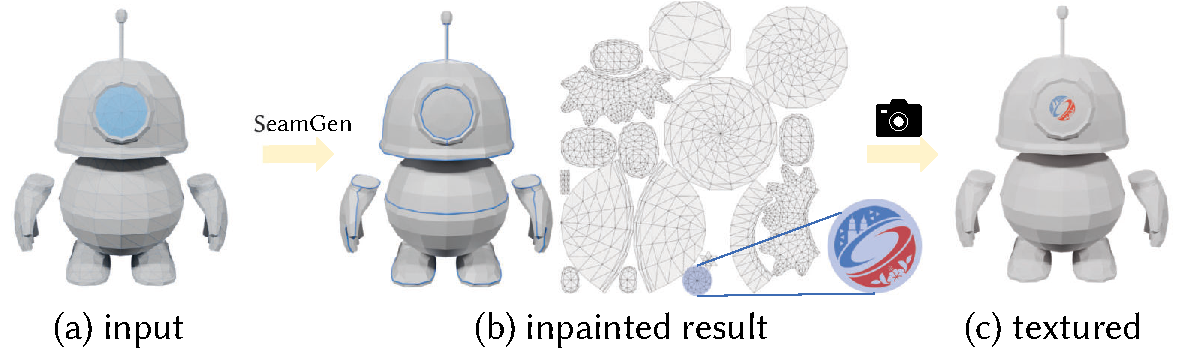
\includegraphics[width=\columnwidth]{figures/user_guide_vis.pdf}
    \caption{
    \textbf{User-guided seam generation via conditional inpainting.}
    (a) The user marks a seam-free region (blue) on the eye area of the mesh, specifying that this region should remain free of cuts.
    (b) Our method completes the remaining seam layout under this constraint and unwraps the mesh into a UV atlas.
    (c) The resulting seam-free eye region provides a clean, continuous surface for texture placement. We insert the SIGGRAPH Asia logo into the corresponding UV region and render the textured result.
    }
    \vspace{-4mm}
    \label{fig:user_guide_vis}
\end{figure}
\subsection{Additional Qualitative Results}
\label{sec:additional_results}

We further demonstrate two practical properties of \methodname{} in production-oriented UV workflows.
First, \methodname{} can preserves structural symmetry when generating seam layouts for symmetric objects. 
As shown in Fig.~\ref{fig:sym}, the generated seams are likely to be placed on corresponding symmetric parts, producing UV islands with compatible shapes after repacking. 
This makes it possible to reuse the same UV space across symmetric regions, improving texture-space utilization and providing a convenient basis for downstream UV-space texture generation and editing. 
We further demonstrate this benefit by generating image textures on the repacked UV layouts using GPT-Image-2~\cite{openai2026gptimage2}.
Second, we evaluate \methodname{} in a component-wise UV unwrapping workflow for complex production assets. 
Although our model is primarily designed for meshes with moderate triangle counts, it can be directly applied to complex models after they are decomposed into semantic components, as commonly done by artists in professional pipelines. 
Fig.~\ref{fig:part} shows an example game asset separated into multiple parts, such as the head, outfit, and accessories. 
Applying \methodname{} to each component produces coherent seam layouts across the full asset, demonstrating its compatibility with practical artist workflows.


\subsection{Conditional Inpainting Applications}
\label{sec:app_inpainting}
We demonstrate the practical utility of conditional seam refinement via the inpainting mechanism introduced in Sec.~\ref{sec:inpainting}.
First, Fig.~\ref{fig:user_guide_vis} demonstrates constraint-guided seam generation. 
Given a user-specified region where seams should be avoided, \methodname{} respects this constraint and completes the remaining cuts into a coherent seam layout. 
This provides simple local control while producing UV layouts suitable for subsequent texture painting.
Second, Fig.~\ref{fig:refinement_vis} shows that the same conditional sampling mechanism can be used for automatic self-refinement. 
When a sampled seam layout produces overlapping UV triangles, \methodname{} locally repairs the problematic region either by adding seams inside the overlapping island or by resampling its boundary together with neighboring islands. 
This corrects many invalid layouts without discarding the entire sample or training an additional repair model. 
Quantitatively, the single-sample predicted overlap rate is reduced from 26.5\% to 3.5\%, demonstrating improved atlas validity.
The detailed refinement procedure is provided in the supplementary material.
% Second, the same mechanism can be used for automatic self-refinement. When a sampled layout produces overlapping UV triangles after parameterization, we fix the reliable parts of the layout and resample only a local region around the problematic island. As illustrated in Fig.~\ref{fig:refinement_vis}, this can be performed either by introducing additional seams inside the overlapping island or by jointly re-sampling the island boundary together with its neighboring islands. This allows the model to correct many invalid samples without discarding the entire layout or training a separate repair model. Quantitatively, this self-refinement procedure reduces the predicted overlap rate from 26.5\% to 3.5\%, demonstrating its effectiveness in improving atlas validity. The concrete refinement procedure and local region selection strategy are provided in the supplementary material.



\begin{figure}[t]
    \centering
    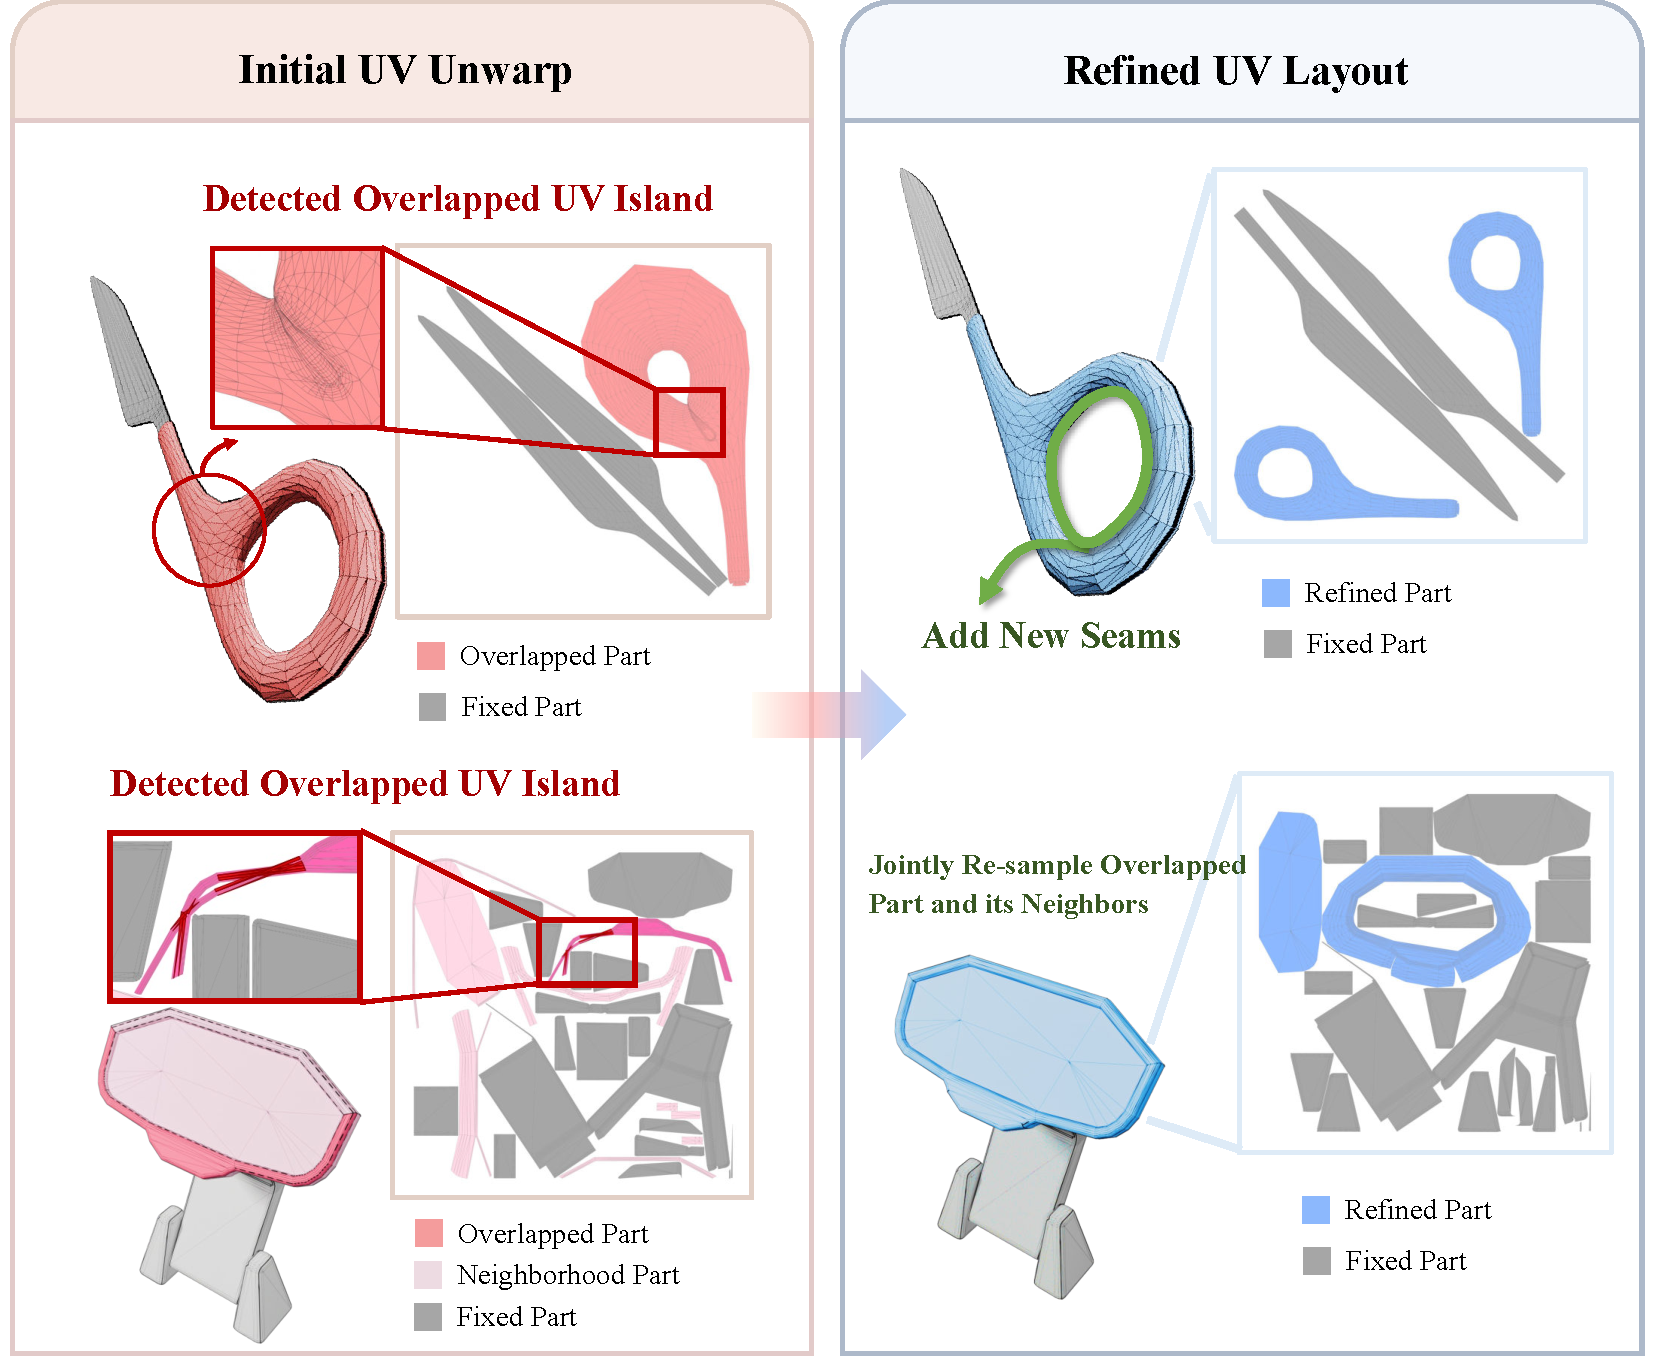
\includegraphics[width=0.99\columnwidth]{figures/uv_refinement.pdf}
    \vspace{-1mm}
    \caption{
    \textbf{Self-refinement via conditional seam inpainting.}
    % Left: initial seam layouts with overlapping UV islands (red).
    % Top: interior-only refinement adds a new seam inside the problematic island.
    % Bottom: boundary-aware refinement jointly resamples the overlapping island and its neighboring islands (yellow).
    % Right: refined, overlap-free UV islands are shown in blue, with newly added seams highlighted in red on the mesh.
    Left: initial layouts with detected overlapping UV islands (red) and their neighborhood (pink). Right: refined, overlap-free UV islands (blue) with updated seam. Top: interior refinement adds new seams (green) within the problematic island. Bottom: boundary-aware refinement jointly resamples the overlapping island and its neighbors. 
    }
    \vspace{-2mm}
    \label{fig:refinement_vis}
\end{figure}

% We evaluate both the architectural design of our Mesh Transformer backbone and the effect of inference-time self-refinement. For the backbone, we consider two variants: \emph{w/o Global Attn}, which removes all global self-attention modules and propagates information purely through the local stream along the mesh connectivity; and \emph{Naive GraphConv}, which keeps the global self-attention stream but replaces the local attention module with a vanilla graph convolution. Since some form of local message passing along mesh edges is structurally necessary for injecting topology, we replace this stream rather than removing it entirely. For a fair comparison, all backbone variants, including the full model, are trained from scratch on the same dataset for 100 epochs under identical optimization settings.

% In addition, we report an inference-time variant, \emph{self-refined}, which uses the full trained model with automatic self-refinement and directly evaluates the initially sampled seam layout. Comparing this variant with the full pipeline measures the effectiveness of the conditional inpainting mechanism when used for automatic overlap correction. All variants are evaluated on the same 200-mesh validation set used in Sec.~\ref{sec:quantitative}. As the evaluation metric, we report the predicted overlap rate, defined as the fraction of meshes whose generated seam layouts produce overlapping UV triangles after flattening; lower is better.

% We ablate both the architectural design of our Mesh Transformer backbone and the inference-time overlap resolution procedure introduced in Sec.~\ref{sec:refinement}. Specifically, we consider three variants: \emph{w/o inpainting}, which uses the full trained model but disables the progressive overlap resolution at inference and reports the single-shot generation result; \emph{w/o Global Attn}, which removes all global self-attention modules and propagates information purely through the local stream along the mesh connectivity; and \emph{Naive GraphConv}, which keeps the global self-attention stream but replaces the local attention module with a vanilla graph convolution. Since some form of local message passing along mesh edges is structurally necessary for injecting topology, we replace this stream rather than removing it entirely. For a fair comparison, all backbone variants, including the full model, are trained from scratch on the same dataset for 100 epochs under identical optimization settings. The \emph{w/o inpainting} variant shares the trained full-model weights and differs only at inference time. All variants are evaluated on the same 200-mesh validation set used in Sec.~\ref{sec:quantitative}. As the evaluation metric, we report the predicted overlap rate, defined as the fraction of meshes whose generated seam layouts produce overlapping UV triangles after flattening; lower is better.

% Our progressive overlap-resolution strategy substantially improves the validity of generated seam layouts at inference time. Starting from the base model predictions, the proposed two-stage inpainting procedure reduces the overlap rate to 3.5\%, successfully resolving roughly seven out of eight overlapping cases without any additional training. This shows that most invalid samples do not need to be discarded and regenerated from scratch, but can instead be corrected through localized conditional seam refinement. For a clean architectural comparison, we next focus on the backbone variants without inpainting. Removing the global self-attention stream increases the overlap rate to 48.1\%, indicating that long-range communication is important for producing globally coherent seam layouts. Replacing the local attention stream with a naive graph convolution is even more detrimental, raising the overlap rate to 72.6\%. This suggests that expressive local modeling is the most critical component of the backbone. Unlike local attention, a simple graph convolution cannot adaptively emphasize geometrically salient neighboring edges, and therefore captures fine-scale seam cues much less effectively. Overall, these ablations show that the local and global streams play complementary roles: the local stream anchors seams to geometrically meaningful boundaries, while the global stream promotes consistency across distant mesh regions. Built on top of this backbone, our progressive inpainting strategy further improves robustness by repairing the remaining overlap failures at inference time, yielding the lowest final overlap rate among all variants.
% We ablate both the architectural design of our Mesh Transformer backbone and the inference-time overlap resolution procedure introduced in Sec.~\ref{sec:refinement}. We consider three variants: w/o inpainting, which uses the full trained model but disables the progressive overlap resolution at inference and reports the single-shot generation result; w/o Global Attn, which removes all global self-attention modules and propagates information purely along the mesh connectivity through the local stream; and Naive GraphConv, which keeps the global self-attention stream but replaces the local attention module with a vanilla graph convolution, since some form of local message passing along the mesh edges is structurally necessary to inject topology, we substitute rather than remove this stream. All variants, including the full model, are trained from scratch on the same dataset for 100 epochs under identical optimization settings for a fair comparison; the w/o inpainting  variant shares the trained full-model weights and differs only at inference. All variants are evaluated on the 200-mesh validation set used in Sec.~\ref{sec:quantitative}. We measure structural quality via the \textbf{predicted overlap rate}, defined as the fraction of meshes whose generated seam layout produces overlapping triangles after flattening; lower is better.





% Disabling the progressive overlap resolution at inference (\emph{w/o inpainting}) raises the predicted overlap rate from 3.5\% to 26.5\%, since every failure must be salvaged by redrawing a fresh noise sample rather than locally repaired; the two-stage inpainting procedure recovers roughly seven out of eight of these failures without any additional training. Among the backbone ablations, which likewise skip inpainting for a clean architectural comparison, removing the global self-attention stream raises the predicted overlap rate from 26.5\% to 48.1\%: without long-range communication, seams initiated on one side of the mesh fail to coordinate with those on the opposite side, so UV islands more often wrap around the surface and self-intersect after flattening. Replacing the local attention with a naive graph convolution is even more damaging---the predicted overlap rate jumps to 72.6\%---indicating that an expressive local stream is in fact the most critical component of the backbone. The simpler graph convolution cannot adaptively weight neighboring edges by their geometric salience, so the network loses the fine-grained cues (dihedral angles, local curvature, proximity to sharp creases) that anchor seams to natural boundaries, and the resulting cuts drift away from geometrically meaningful edges; the global stream alone is unable to compensate for this loss of local precision. Only the full model, in which local attention and global self-attention interleave in every block and the progressive inpainting salvages residual overlap, attains the lowest overlap rate, confirming that the two backbone streams are complementary and that the inference-time inpainting further strengthens the pipeline end-to-end.

% Our progressive overlap-resolution strategy is highly effective at repairing invalid seam layouts at inference time. Starting from the base model predictions, the proposed two-stage inpainting procedure reduces the overlap rate to 3.5\%, successfully resolving roughly seven out of eight overlapping cases without any additional training. This shows that most failures do not require discarding the entire sample; instead, they can be corrected through localized conditional seam refinement, making the overall pipeline substantially more reliable in practice.

% For a clean comparison of backbone architectures, we evaluate the following model variants without inpainting. Removing the global self-attention stream increases the overlap rate to 48.1\%, indicating that long-range communication is important for producing globally coherent seam layouts. Without global context, seam decisions made in one region cannot coordinate well with distant regions on the mesh, so the resulting UV islands are more likely to wrap around the surface inconsistently and self-overlap after flattening.

% Replacing the local attention stream with a naive graph convolution is even more detrimental, leading to an overlap rate of 72.6\%. This suggests that expressive local modeling is the most critical component of the backbone. Unlike local attention, a simple graph convolution cannot adaptively emphasize geometrically salient neighboring edges, and therefore captures fine-scale seam cues much less effectively. As a result, the model becomes less sensitive to dihedral angles, local curvature, and proximity to sharp creases, causing seams to drift away from natural cut boundaries. In this case, global communication alone is insufficient to compensate for the loss of local geometric precision.

% Overall, these ablations show that the local and global streams play complementary roles: the local attention stream anchors seams to geometrically meaningful boundaries, while the global self-attention stream promotes consistency across distant mesh regions. Built on top of this backbone, our progressive inpainting strategy further improves robustness by repairing the remaining overlap failures at inference time, yielding the lowest final overlap rate among all variants.
